\documentclass[border=3pt]{standalone}
% Preâmbulo compartilhado pelos diagramas TikZ da aula 12 (Mapeamento por Grade de Ocupação)
\usepackage[T1]{fontenc}
\usepackage[utf8]{inputenc}
\usepackage{lmodern}
\usepackage{amsmath}
\usepackage{xcolor}
\usepackage{tikz}
\usetikzlibrary{arrows.meta,angles,quotes,decorations.pathmorphing,calc,
                positioning,shapes.geometric,shapes.misc,backgrounds,fit,
                math}

% Paleta (mesma dos SVGs originais)
\definecolor{dblue}{HTML}{2A5B8C}
\definecolor{dorange}{HTML}{B3541E}
\definecolor{dgreen}{HTML}{4A7C59}
\definecolor{dred}{HTML}{9C4B4B}
\definecolor{dcream}{HTML}{F4F1EA}
\definecolor{dshade}{HTML}{DDD7C9}

% Função gaussiana (não normalizada por padrão de escala visual)
\pgfmathdeclarefunction{gauss}{3}{%
  \pgfmathparse{1/(#3*sqrt(2*pi))*exp(-((#1-#2)^2)/(2*#3^2))}%
}

% Estilos comuns (prefixo d... para não colidir com chaves internas do pgf)
\tikzset{
  >={Stealth[length=2mm]},
  dguide/.style={gray!55, dashed, line width=0.4pt},
  daxis/.style={gray!60, line width=0.7pt, ->},
  dbody/.style={fill=black!3, draw=black!80, line width=1pt},
  dacc/.style={draw=dblue, line width=1pt},
  dlbl/.style={black!55, font=\small},
  dsub/.style={black!45, font=\footnotesize},
  dstate/.style={circle, draw=black!80, fill=dcream, line width=1pt,
                 minimum size=17mm, font=\large, inner sep=1pt},
  dobs/.style={circle, draw=black!80, fill=dshade, line width=1pt,
               minimum size=14mm, font=\large, inner sep=1pt},
  dbox/.style={rounded corners=2pt, draw=black!80, fill=dcream, line width=1pt,
               align=center, inner sep=6pt},
  dop/.style={circle, draw=black!80, fill=white, line width=1pt,
              minimum size=6mm, inner sep=0pt, font=\small},
  dtrans/.style={->, dblue, line width=1pt},
  dmeas/.style={->, dorange, line width=1pt},
  dcurve/.style={line width=1pt, dblue},
  dcurveb/.style={line width=1.4pt, dorange},
}

\begin{document}
\hyphenpenalty=10000 \exhyphenpenalty=10000 \tolerance=9999 \emergencystretch=3em
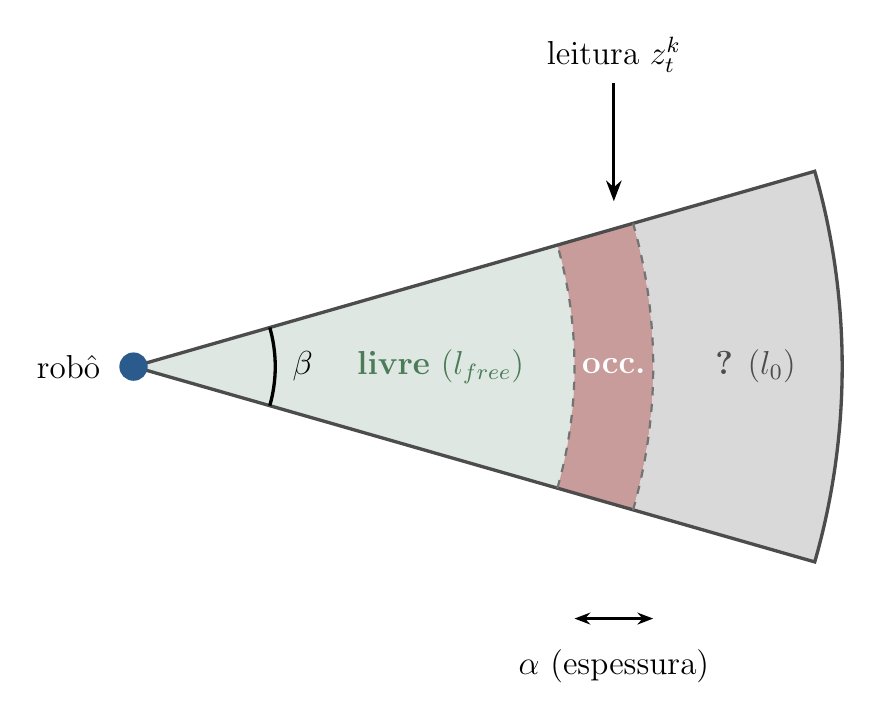
\begin{tikzpicture}[x=1cm,y=1cm]
  \def\bw{16}
  \fill[dgreen!18] (0,0) -- (-\bw:5.6) arc(-\bw:\bw:5.6) -- cycle;
  \fill[dred!55] (-\bw:5.6) arc(-\bw:\bw:5.6) -- (\bw:6.6) arc(\bw:-\bw:6.6) -- cycle;
  \fill[black!15] (-\bw:6.6) arc(-\bw:\bw:6.6) -- (\bw:9.0) arc(\bw:-\bw:9.0) -- cycle;
  \draw[black!70, line width=1.2pt] (0,0) -- (-\bw:9.0) arc(-\bw:\bw:9.0) -- cycle;
  \draw[black!55, dashed, line width=0.8pt] (-\bw:5.6) arc(-\bw:\bw:5.6);
  \draw[black!55, dashed, line width=0.8pt] (-\bw:6.6) arc(-\bw:\bw:6.6);
  \fill[dblue] (0,0) circle (0.18); \node[font=\large, anchor=east] at (-0.3,0) {robô};
  \node[font=\large, dgreen] at (3.9,0) {\textbf{livre} ($l_{free}$)};
  \node[font=\large, white] at (6.1,0) {\bf occ.};
  \node[font=\large, black!70] at (7.9,0) {\textbf{?} ($l_0$)};
  \draw[<->, line width=1.2pt] (5.6,-3.2) -- (6.6,-3.2); \node[font=\large] at (6.1,-3.8) {$\alpha$ (espessura)};
  \draw[line width=1.2pt] (-\bw:1.8) arc(-\bw:\bw:1.8);
  \node[font=\large] at (2.15,0) {$\beta$};
  \draw[-{Stealth}, line width=1pt] (6.1,3.6) node[above, font=\large] {leitura $z_t^k$} -- (6.1,2.1);
\end{tikzpicture}
\end{document}
